%%%%%%%%%%%%%%%%%%%%%%%%%%%
\chapter {Background and Related Work}
\label{BRW}
%%%%%%%%%%%%%%%%%%%%%%%%%%%
\section{Mobile Ad hoc Networks}
\noindent ``Ad hoc networks are infrastructure-less and cooperation-based networks which means that the network topologies must be decided by the network sensors themselves'' \cite {C14}. In other words, the major feature of ad hoc networks is that they have no infrastructures.

The Mobile Ad hoc NETwork (MANET), also called the Wireless Ad hoc NETwork (WANET), is a decentralized wireless network with no pre-existing infrastructure. In MANET, because users move independently, the topology changes frequently. Without the help of infrastructure, users can only communicate when they encounter each other. In other words, users communicate only if they are covered by each other's communication range. Because of the above characteristics, the MANET can be viewed as a kind of Delay-Tolerant Network (DTN) that lacks continuous network connectivity. The MANET can hardly establish instantaneous end-to-end paths, which compels the routing protocols in MANET to use a ``store-and-forward'' strategy in which users forward messages when they encounter others, or they store messages for later delivery. As shown in Figure \ref{fig:MANET}, the user $A$ has a message for $C$ but does not know where $C$ is, so he sends the message to $B$ when they encounter each other. The user $B$ then stores the message and moves along. The message is then delivered to $C$ when both $B$ and $C$ come in contact with each other at a later time. It is obvious that whether the message can be delivered depends on the movement of the users. If $B$ will never meet $C$ or the message is held by a user for a long period of time, it must be dropped after some timeout. The delivery process can lead to low success ratio and is often time-consuming.

\begin{figure} [H]
  \centering 
  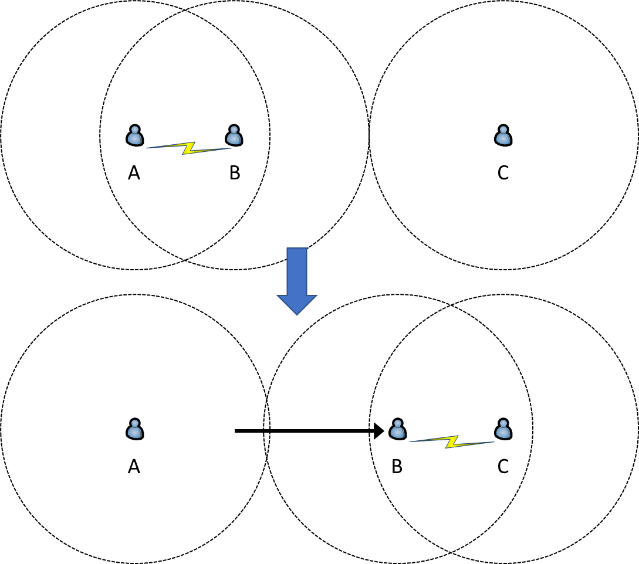
\includegraphics[width=4.0in]{figures/FIG_MANET.png}
  \caption{MANET} 
  \label{fig:MANET} %% label for entire figure 
\end{figure}

\section{Delay Tolerant Network}

\noindent Regular networks, e.g. Internet, always have end-to-end paths. As shown in Figure \ref{fig:comparison_RN_DTN:a}, two nodes $S$ and $D$ are connected through nodes $A$, $B$, and $C$. The maximum round-trip time is not excessive, and their drop probability is also small. Compared to the regular network, there is a class of challenged networks \cite {C1} which lack end-to-end path and suffer from high latency and long queuing delays. As shown in Figure \ref{fig:comparison_RN_DTN:b}, when node $B$ is down or non-existent, there is no connection between nodes $A$ and $C$, for which extensive latency is inevitable if the source $S$ sends a message to the destination $D$.

\begin{figure} [H]
  \centering 
  \subfigure[Regular Network]{ 
    \label{fig:comparison_RN_DTN:a} %% label for first subfigure 
    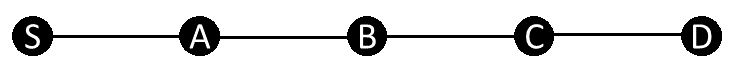
\includegraphics[width=4.0in]{figures/FIG_Regular_Network.png}} 
  \hspace{1in} 
  \subfigure[DTN]{ 
    \label{fig:comparison_RN_DTN:b} %% label for second subfigure 
    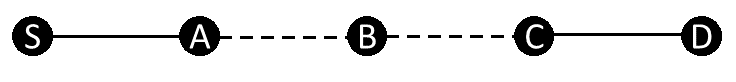
\includegraphics[width=4.0in]{figures/FIG_DTN.png}}
  \caption{The comparison between regular networks and DTNs} 
  \label{fig:comparison_RN_DTN} %% label for entire figure 
\end{figure}

Since the challenged networks are significantly different from the regular networks, researchers have introduced a new architecture, called Delay Tolerant Network (DTN), to deal with the unique features of the challenged networks. Terrestrial Mobile Networks, Exotic Media Networks, Military Ad Hoc Networks and Sensor/Actuator Networks are examples of typical DTNs.


\subsection{ Spray and Wait Protocol}

\noindent The Spray and Wait \cite{C31} is a well-known protocol for message dissemination in DTNs. Although it is not as efficient as protocols on Internet, it works quite well in DTNs. A message is initialized with several copies, a part of which are given to others when users encounter each other. Users keep forwarding copies until they each have only one copy of the message. When a user carrying at least one copy of the message encounters the destination, he gives all his copies to the destination to complete the delivery. The Binary Spray and Wait (BSW) \cite{C31} is an optimized version of the Spray and Wait, which we use for comparison in this thesis. The user who creates the message also makes several copies of that message. He gives half of his copies to the user whom he encounters so that both he and the other user have half of the copies. The users who get copies of the message continue to give half of their copies to others until someone has only one copy to pass on to the destination.

\subsection{ Other DTN Protocols}


\subsubsection{ Direct Contact Scheme}

\noindent The simplest strategy for DTN is that the source holds the message until he meets the destination, which is called the direct contact scheme. So, a direct path between the source and the destination is necessary for a successful delivery. It is possible that the source never comes in contact with the destination in which case the message is not delivered. 


\subsubsection{ Replica Based Protocols}

\noindent The replica based protocols (e.g., \cite{C6}, \cite{C7}, \cite{C8}, \cite{C9}, and \cite{C37}) work by making several replicas of the message so that users can retransmit them upon connection establishment. The former BSW is also a kind of replica based protocols. Compared to the direct contact scheme, the replica-based protocols make it easy for messages to be delivered. But, they require more resources than the direct contact scheme because they need more memory to store the replicas. Therefore, making a reasonable decision on the message replication is the key to success of these kinds of protocols.


\subsubsection{  Knowledge-Based Protocols}

\noindent Different from the former replica protocols which require no knowledge about the topology of the network, the users in knowledge-based protocols try to evaluate their own view of the topology of the network so that they can make better forwarding decisions, e.g. \cite{C36}, \cite{C38} and \cite{C39}. However, the topology changes so frequently that it is hard for users to have an accurate topology.


\subsubsection{ Coding Based Protocols}

\noindent Authors in \cite {C12} and \cite {C13} have suggested the approach that introduces coding techniques into the routing protocols. Instead of making a few replicas, coding based protocols encrypt data to make a large number of message blocks. If the destination receives a part of the blocks, he can decrypt the message.

\section{Location-Based Services}

\noindent The Location-Based Services (LBS) use users' location information to provide services as shown in Figure \ref{fig:LBS}. Your smartphone can detect your coordinate and send it to LBS application server which is responsible for providing service based on the coordinate. The point of interest and the location advertisement are familiar instances of LBS. The LBS providers collect users' location information to provide service, which makes LBS providers a significant target of attack. When attackers access the databases of the LBS providers, they can learn all sensitive information in the servers. So, the LBS providers should be viewed as semi-trusted, which might expose information in front of vicious attackers.

Users face risks of information breach when they access a semi-trusted LBS provider because anyone who has access to data in LBSs is able to steal and misuse LBS users' location-privacy. Considering that LBSs rely on location-aware computing, it is unavoidable to leak users' location from LBSs. Therefore, balancing ``these two competing aims of location privacy and location awareness'' \cite {C20} is always a challenge.

\begin{figure} [H]
  \centering 
  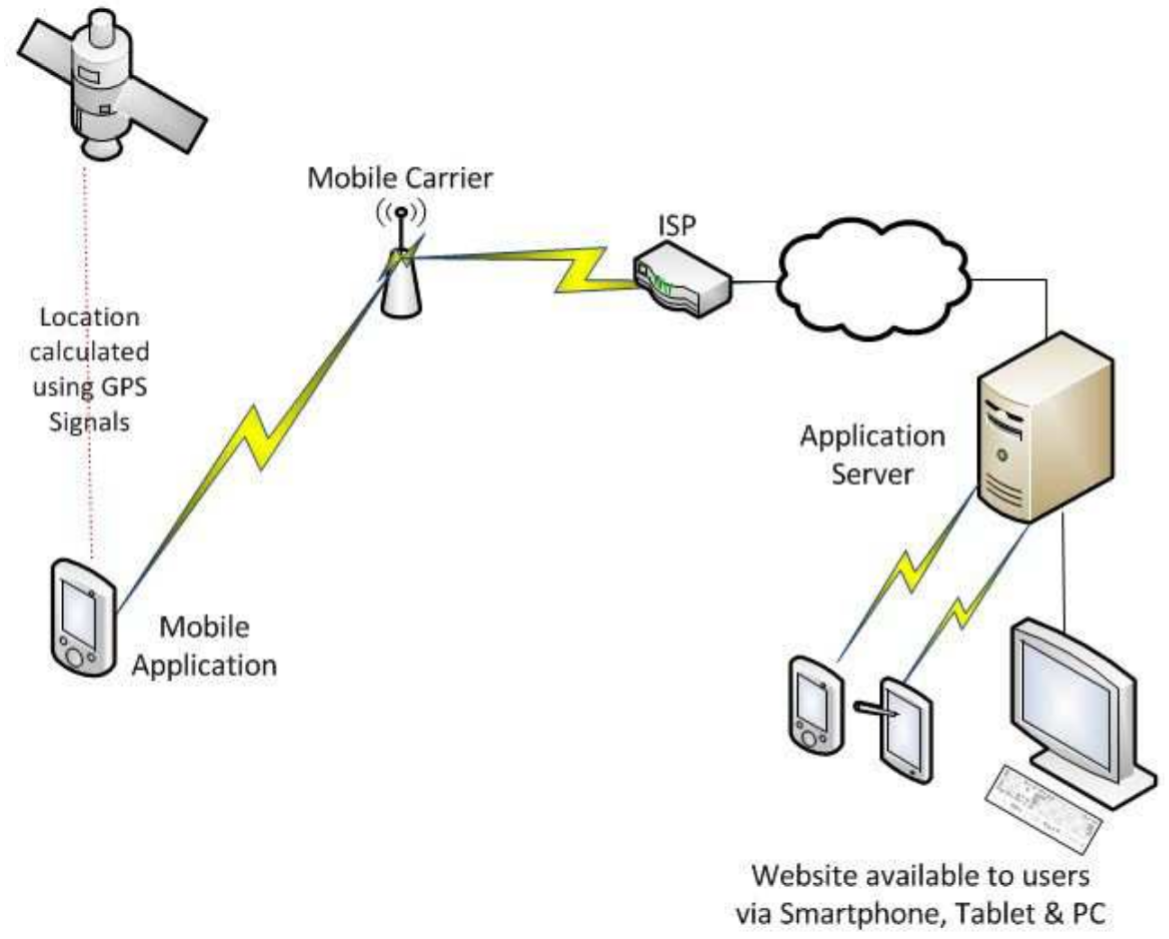
\includegraphics[width=4.0in]{figures/FIG_LBS_11.png}
  \caption{LBS \cite {C11}} 
  \label{fig:LBS} %% label for entire figure 
\end{figure}

\section{Social Networks}

\noindent Social networks which contain social interactions and personal relationships are used in location-privacy protection so that users can determine who can or cannot be trusted. In \cite {C30}, the relationship of a pair of people (e.g., user $i$ and user $j$) is described as a pair of directed relationship strength. The directed relationship strength from the user $i$ to the user $j$ can be denoted by ${RS}^{ij}$. We should notice that ${RS}^{ij}$ might not be equal to ${RS}^{ji}$, because the user $i$ might like the user $j$ very much while the user $j$ just views the user $i$ as an acquaintance. Based on the relationship strength, it is possible to estimate the relational tie between two people and predict whether they are friends or strangers. 

The relationship strength is compared with a threshold; if the relationship strength is higher than the threshold then the two people are friends, otherwise they are strangers. In the protocols we mention in the thesis, researchers always assume that friends are trustful. That is reasonable because you might feel more secure when your friends forward your message instead of a stranger. 


\section{Location-Privacy Protocols}

\noindent The basic idea of most location-privacy protocols is hiding the original requester behind a set of users so that attackers can hardly infer the identity of the original requester. In other words, when a user sends a query, his identity cannot be inferred based on the information in the query easily. For example, the original requester can use a pseudonym instead of his real name or use an obfuscated location to send his queries, so that attackers cannot tell the difference between two sets of queries. 

The location-privacy protocols are considered centralized and distributed based on whether they require any infrastructure for operation. 


\subsection{ Centralized Protocols}

\noindent Centralized protocols always need some infrastructure for the obfuscation process. The infrastructure could be any equipment which acts as an anonymization server. When the user wants to send a query to the LBS server, he sends the query to the anonymization server. The anonymization server changes the identity and the location in the query, which is called anonymization or obfuscation. Then, the anonymization server forwards the modified query to the LBS server, so that the attacker who attacks the LBS server can hardly learn the identity of the original requester. The LBS server can send the reply message to the anonymization server which is responsible for forwarding the reply message back to the original requester. In this way, the original requester gets the information he needs, while avoiding from being located by the attackers.

The advantage of a centralized protocol is that the anonymization server has more resources and information than users in the network, which enable the server to achieve better anonymization performance and provide sufficient protection for users. For example, if the anonymization server knows locations of all users in the network, it can modify the location and identity in the queries to the most suitable, with which the LBS server can provide acceptable results while the original requester is not exposed.

There are two major shortcomings of these kinds of protocols: i) it is hard to deploy infrastructure in some areas, ii) since the anonymization server knows users' location, it is also a risk for the users.


\subsubsection{ Single Server}

\noindent Authors in \cite {C15} use a central anonymity server through which the mobile users can send queries to LBS. To make the communication between users and the central anonymity server trustful, users set up an encrypted connection with the anonymity server at the beginning. Users sends their encrypted queries to the anonymity server, so that the anonymity server is the only one who can learn the information in the query. The anonymity server decrypts the queries and uses a cloaking algorithm to perturb the position information in the queries. Then the anonymity server sends the modified queries to external services (e.g., LBS). This is a typical centralized protocol, which can reduce the re-identification risk for the users. Its drawback is that a continuous connection to the server is necessary for each user, which is hard to achieve in a sparse DTN. We cannot also assume that a MANET user can have a stable connection with a central anonymity server either.

In \cite {C23}, researchers employ a matchmaker which is used to match users and advertisements, by which users can achieve anonymization of their identities and locations from the matchmaker. The system architecture in \cite {C23} is similar to the former \cite {C15}, while authors in \cite {C23} just focus on the advertisement service instead of the ``external services'' in \cite{C15}. The role of the matchmaker is simply matching users and advertisements. Although the functions of the matchmaker in \cite {C23} and the central anonymity server in \cite {C15} are different, the intermediate trusted three-party servers (i.e., the matchmaker and the central anonymity server) separate users and the application server (e.g., an advertisement server, LBS server). The architecture in \cite {C23} does not require an encryption process, so the attackers can learn the information in the queries. When a large number of queries arrive at the matchmaker in a short time from different users, it helps the matchmaker mix the queries so that attackers can hardly trace the query, but the burden of the users who are near the matchmaker can be heavy.

In \cite {C24}, researchers use a trusted, third-party location anonymization engine (LAE) that acts as a middle layer between mobile users and the LBS provider, in which exact locations and requests from clients are replaced by a location anonymization engine before they arrive at the LBS provider. Therefore, it appears that the suggest approach is almost like that shown in Figure \ref{fig:SingleAnoymizationServer}. A trusted server is placed between users and the application server, which hides users' information and offers sufficient information for the application servers to provide acceptable service. 

\begin{figure} [H]
  \centering 
  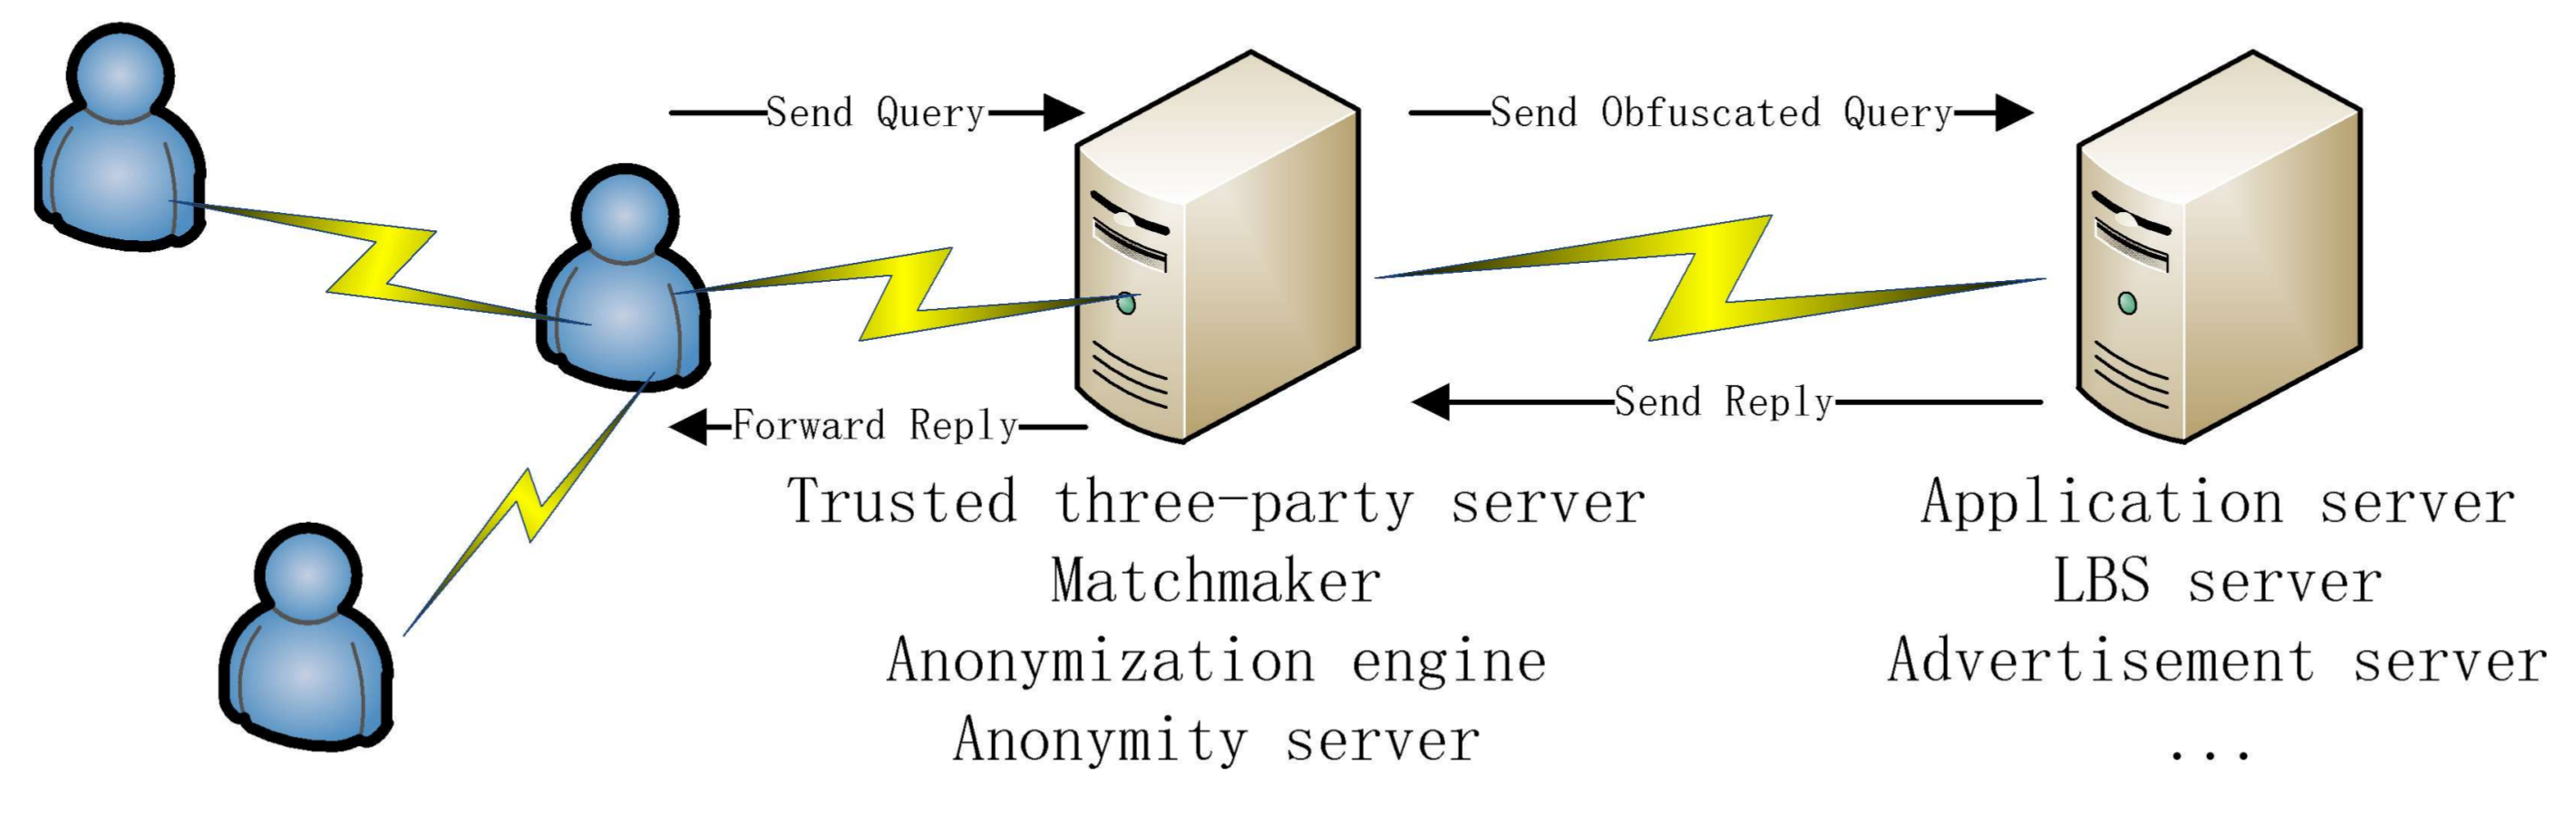
\includegraphics[width=5.0in]{figures/Fig_Single_Ano_Ser.png}
  \caption{Single Anonymization Server} 
  \label{fig:SingleAnoymizationServer} %% label for entire figure 
\end{figure}

\subsubsection{ Multiple Servers}

\noindent The above protocols always use a single anonymization server, while there are other protocols which need multiple infrastructures. 

Authors in \cite{C25} propose a protocol, called Social-based PRivacy-preserving packet forwardING (SPRING), for vehicular delay-tolerant network. In their work, they employ Roadside Units (RSUs), which are a type of equipment deployed along the roadside, to assist the packet forwarding and achieve conditional privacy preservation. These RSUs are located at high social intersections, so that vehicles which pass by the RSUs send their messages to the RSUs. The RSUs have sufficient resource so that they can hold the messages for a long time, which decreases the probability of messages being dropped. The messages are forwarded to proper next-hop vehicles when the vehicles pass by the RSUs. Since messages are held by the RSUs for a period, attackers can hardly trace the messages. Besides, a large number of vehicles send many packets to these RSUs, which enables the RSUs to serve as mix servers. The advantage of SPRING is that it improves the delivery success ratio and privacy-protection performance. However, deploying the RSUs is not always feasible.

Another example is the REAL \cite{C26}, in which researchers use sensor nodes which are scattered throughout the network to provide anonymized locations for users, as shown in Figure \ref{fig:REAL}. The whole system area is partitioned into a set of aggregate locations by the sensor nodes, where there are at least $k$ persons. To provide better location-based service, they minimize the areas of aggregate locations. When a user sends a query to the LBS, he uses the location of the sensor nodes which he belongs to, so that the attacker cannot tell the difference between the requester and the other $k-1$ users in that aggregate location. This is a typical k anonymity algorithm, whose main disadvantage is that it is difficult to deploy the sensor nodes in real-world. Besides, the mix servers and sensor nodes might be more prominent targets than the LBS providers.

\begin{figure} [H]
  \centering 
  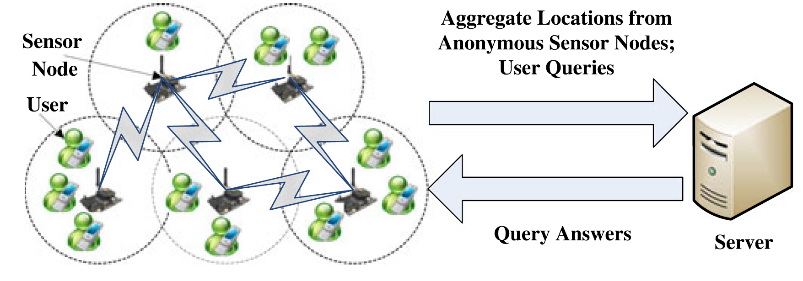
\includegraphics[width=5.0in]{figures/FIG_REAL_26.png}
  \caption{REAL \cite{C26}} 
  \label{fig:REAL} %% label for entire figure 
\end{figure}

\subsection{ Distributed Protocols}

\noindent Although centralized protocols also have good performance in their delivery success ratio and privacy-protection in their own field, the MANET is a network without infrastructure. Distributed protocols are more appropriate for applications in MANET. A problem for a distributed protocol it that whether a user can trust others. Authors in \cite{C16}, \cite{C17} and \cite{C18} introduce the social tie to determine whether a user is trustful.

In the distributed social based location privacy protocol (SLPD) \cite{C16}, authors use two phases: the obfuscation phase and the free phase. A query from an original requester always starts in the obfuscation phase and passes through \textit{k} friends. For example, the original requester sends the query to one of his friend in one hop, then the friend forwards the query to another friend. We call these friends the agents. That process repeats for exactly $k$ times. When the $k^{th}$ friend get the query, he switches the query to the free phase and replaces the sender identity with his own identity, and then sends the query to the destination (e.g., LBS) using any DTN protocol. The LBS then sends the reply to all \textit{k} friends who are responsible for forwarding the message to the original requester. In this way, attackers can only learn the identity of all \textit{k} friends instead of the original requester. Since each of these \textit{k} friends knows the identity of the original requester, the message can be forwarded to the original requestor.  Therefore, the attacker can hardly learn the identity of the original requester. The disadvantage of the protocol is that it is hard to encounter a friend in the network, which can decrease the success ratio for the queries. 
In the protocol, Hybrid and Social-aware Location-Privacy in Opportunistic mobile social networks (HSLPO) \cite{C17}, authors try to improve the delivery performance by using a stochastic model which uses a Markov model for location predication. The major process is similar to that in SLPD, but an agent can forward the query to a user who is not a friend of the original requester if the user has more chance to deliver the query and a trust value is larger than a threshold. In other words, an agent continuously searches his surrounding to find the original requester's friends. If the agent cannot find the original requester's friend but his own friend, he checks whether his friend has more chance to deliver the query than him using the Markov model. If his friend is more suitable for forwarding, he sends the query to his friend. The performance of HSLPO depends on the Markov model, that is, whether it can predict users' movement accurately. In real-world, the movement model for people is more complicated than that used in experiments.

Another protocol, called Location Privacy-Aware Forwarding (LPAF) \cite{C18}, also attempts to improve the performance of SLPD. Both LPAF and SLPD are similar, but LPAF just adds more friends to the protocol. When an agent cannot find a close friend (i.e., their trust value is high), he will try to find other general friends (i.e., their trust values is lower than the close friends). That might be a safety tradeoff, because some ineligible users in SLPD can be chosen as friends based on the additional criteria imposed by LPAF.

In fact, both the HSLPO and LPAF do not successfully address the problem of finding friends as agents. Although we use the friends of friends or set the threshold for friends low, there are only a few users who can be chosen as agents. In LPAF, the identity of the requester is even exposed to someone who is not very trustful. 




















